\documentclass{article}\usepackage[]{graphicx}\usepackage[]{color}
%% maxwidth is the original width if it is less than linewidth
%% otherwise use linewidth (to make sure the graphics do not exceed the margin)
\makeatletter
\def\maxwidth{ %
  \ifdim\Gin@nat@width>\linewidth
    \linewidth
  \else
    \Gin@nat@width
  \fi
}
\makeatother

\definecolor{fgcolor}{rgb}{0.345, 0.345, 0.345}
\newcommand{\hlnum}[1]{\textcolor[rgb]{0.686,0.059,0.569}{#1}}%
\newcommand{\hlstr}[1]{\textcolor[rgb]{0.192,0.494,0.8}{#1}}%
\newcommand{\hlcom}[1]{\textcolor[rgb]{0.678,0.584,0.686}{\textit{#1}}}%
\newcommand{\hlopt}[1]{\textcolor[rgb]{0,0,0}{#1}}%
\newcommand{\hlstd}[1]{\textcolor[rgb]{0.345,0.345,0.345}{#1}}%
\newcommand{\hlkwa}[1]{\textcolor[rgb]{0.161,0.373,0.58}{\textbf{#1}}}%
\newcommand{\hlkwb}[1]{\textcolor[rgb]{0.69,0.353,0.396}{#1}}%
\newcommand{\hlkwc}[1]{\textcolor[rgb]{0.333,0.667,0.333}{#1}}%
\newcommand{\hlkwd}[1]{\textcolor[rgb]{0.737,0.353,0.396}{\textbf{#1}}}%

\usepackage{framed}
\makeatletter
\newenvironment{kframe}{%
 \def\at@end@of@kframe{}%
 \ifinner\ifhmode%
  \def\at@end@of@kframe{\end{minipage}}%
  \begin{minipage}{\columnwidth}%
 \fi\fi%
 \def\FrameCommand##1{\hskip\@totalleftmargin \hskip-\fboxsep
 \colorbox{shadecolor}{##1}\hskip-\fboxsep
     % There is no \\@totalrightmargin, so:
     \hskip-\linewidth \hskip-\@totalleftmargin \hskip\columnwidth}%
 \MakeFramed {\advance\hsize-\width
   \@totalleftmargin\z@ \linewidth\hsize
   \@setminipage}}%
 {\par\unskip\endMakeFramed%
 \at@end@of@kframe}
\makeatother

\definecolor{shadecolor}{rgb}{.97, .97, .97}
\definecolor{messagecolor}{rgb}{0, 0, 0}
\definecolor{warningcolor}{rgb}{1, 0, 1}
\definecolor{errorcolor}{rgb}{1, 0, 0}
\newenvironment{knitrout}{}{} % an empty environment to be redefined in TeX

\usepackage{alltt}
\usepackage{float} 
\usepackage{booktabs}
\usepackage{longtable}
\usepackage{xcolor,colortbl}

\colorlet{tableheadcolor}{gray!50}
\newcommand{\headcol}{\rowcolor{tableheadcolor}}
\colorlet{tablerowcolor}{gray!25}
\newcommand{\rowcol}{\rowcolor{tablerowcolor}}

\usepackage{geometry}
\geometry{verbose, tmargin=2cm, bmargin=2cm, lmargin=2cm, rmargin=2cm}
\IfFileExists{upquote.sty}{\usepackage{upquote}}{}
\begin{document}



\title{Projected Vegetation Change 2009 vs. 2100 \\ \large Unvetted preliminary rush draft from developmental code}
\author{Matthew Leonawicz}
\maketitle

\setlength{\aboverulesep}{0.2pt}
\setlength{\belowrulesep}{0.2pt}





\section{Area Trends by Vegetation Class and Scenario}
The below graph relates to figure 6.3 in the original document.
This uses strictly ALFRESCO output.
\subsection{Alaska}
\begin{figure}[H]
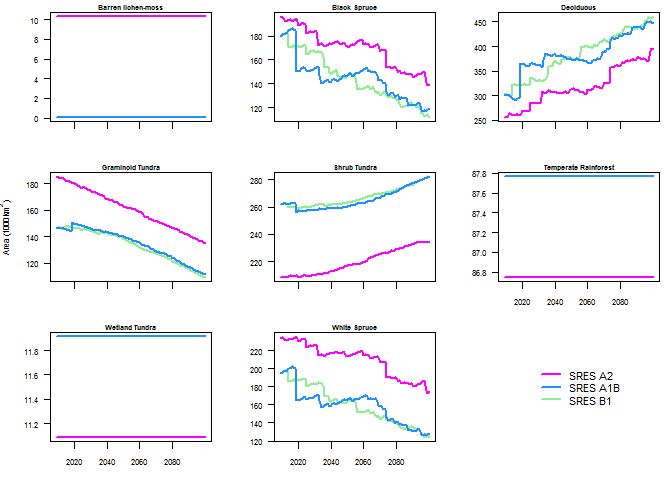
\includegraphics[width=\maxwidth]{figure/veg_change_ts_AK-1} \caption[Alaska]{Alaska\label{fig:veg_change_ts_AK}}
\end{figure}



All five following separate LCC graphs relate to figure 6.3 in the original document.
This uses strictly ALFRESCO output.
\subsection{Arctic}
\begin{figure}[H]
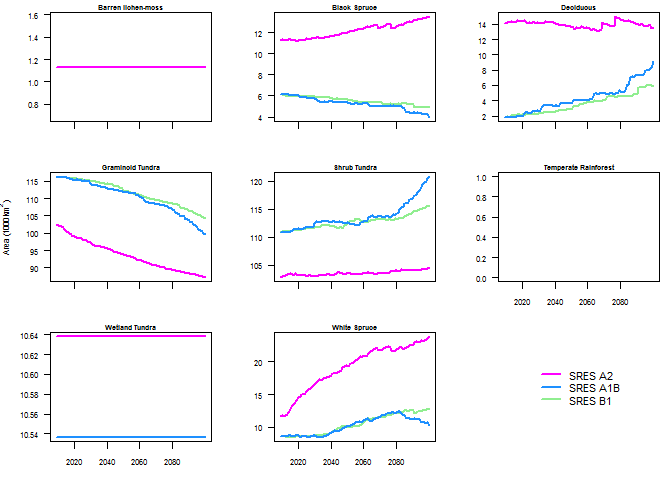
\includegraphics[width=\maxwidth]{figure/veg_change_ts_LCC1-1} \caption[Arctic]{Arctic\label{fig:veg_change_ts_LCC1}}
\end{figure}



\subsection{North Pacific}
\begin{figure}[H]
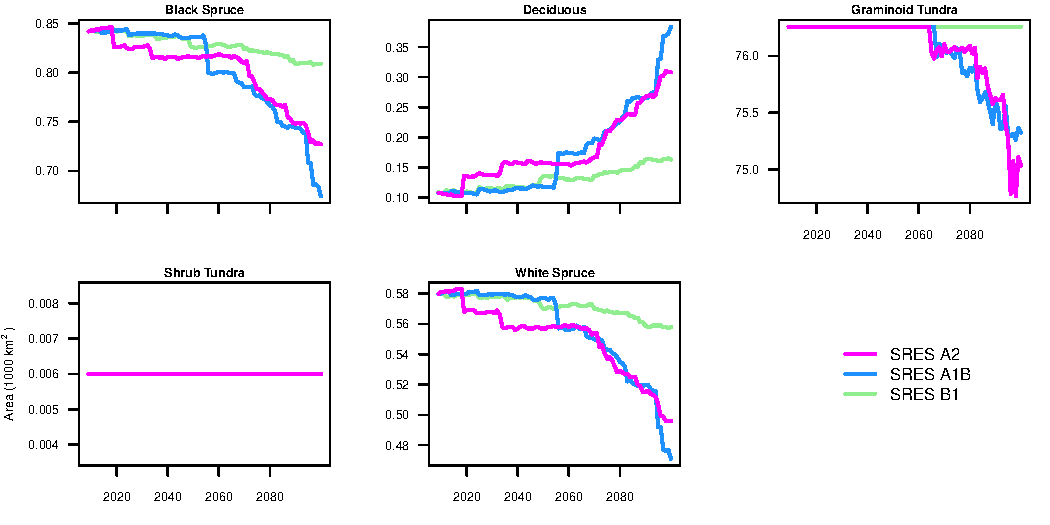
\includegraphics[width=\maxwidth]{figure/veg_change_ts_LCC2-1} \caption[North Pacific]{North Pacific\label{fig:veg_change_ts_LCC2}}
\end{figure}



\subsection{Northwest Interior Forest North}
\begin{figure}[H]
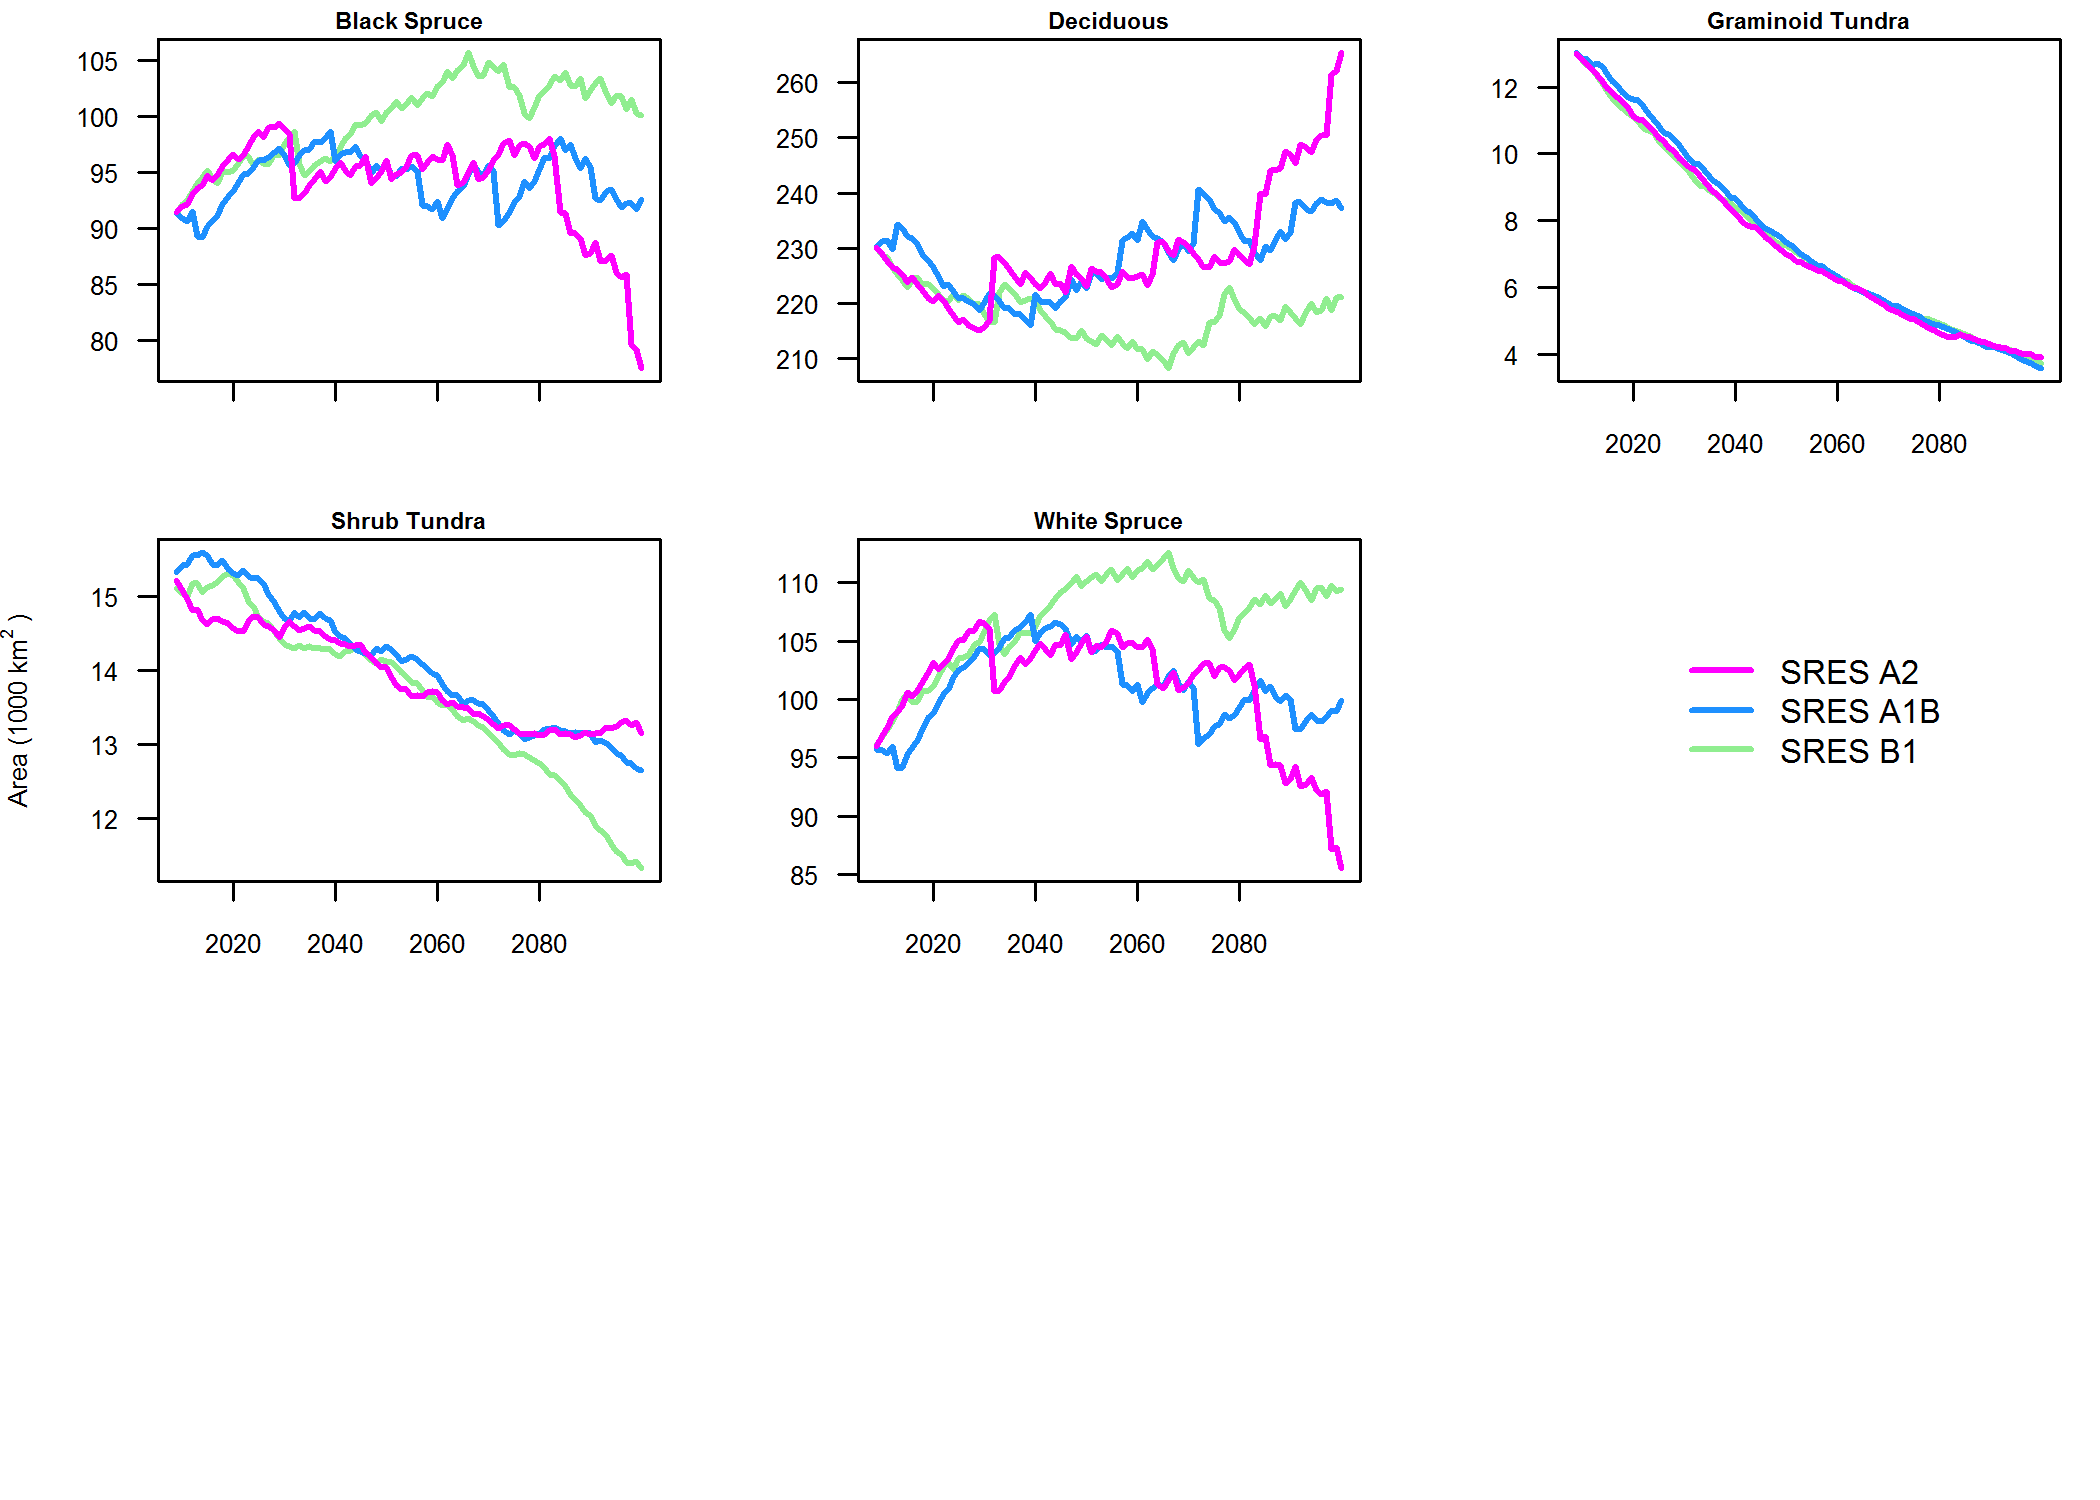
\includegraphics[width=\maxwidth]{figure/veg_change_ts_LCC3-1} \caption[Northwest Interior Forest North]{Northwest Interior Forest North\label{fig:veg_change_ts_LCC3}}
\end{figure}



\subsection{Northwest Interior Forest South}
\begin{figure}[H]
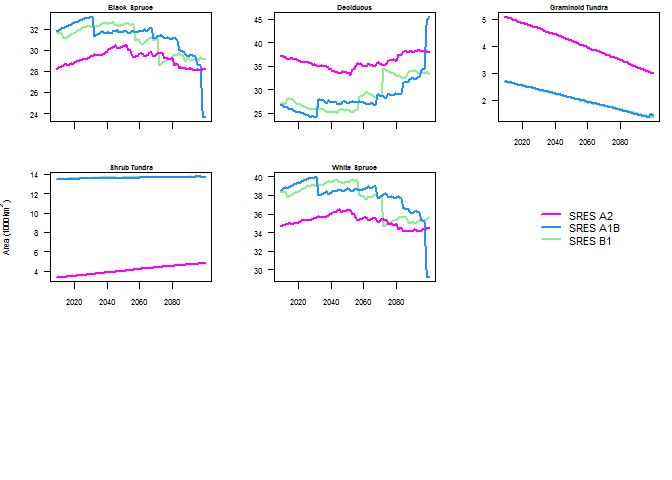
\includegraphics[width=\maxwidth]{figure/veg_change_ts_LCC4-1} \caption[Northwest Interior Forest South]{Northwest Interior Forest South\label{fig:veg_change_ts_LCC4}}
\end{figure}



\subsection{Western Alaska}
\begin{figure}[H]
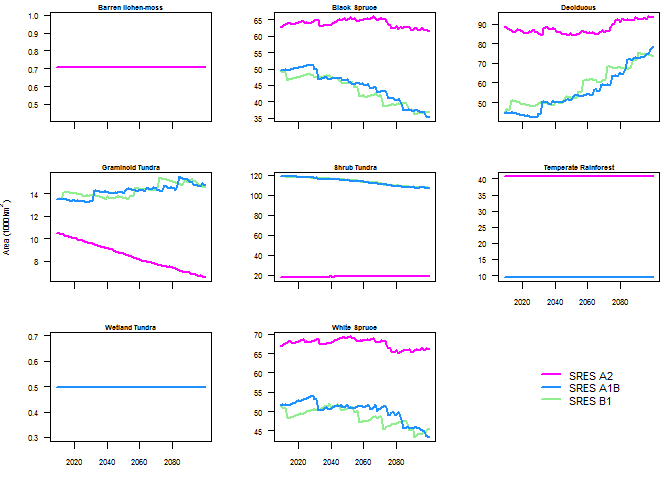
\includegraphics[width=\maxwidth]{figure/veg_change_ts_LCC5-1} \caption[Western Alaska]{Western Alaska\label{fig:veg_change_ts_LCC5}}
\end{figure}



\end{document}
